\documentclass[twocolumn]{article}
\usepackage[spanish]{babel}
\usepackage[utf8]{inputenc}
\usepackage{amsmath}
\usepackage{natbib}
\usepackage{microtype}
\usepackage{etoolbox}
\usepackage{amssymb}
\usepackage{graphicx}
\usepackage{lipsum}
\usepackage{fancyhdr}
\usepackage{abstract}
\usepackage{geometry}
\usepackage{booktabs}
%Ubicacion de los graficos 
\graphicspath{ {imagenes/} }

% DEFINIR LOS COMANDOS QUE FALTAN
\providecommand{\apjs}{ApJ Suppl. Ser.}
\providecommand{\aj}{Astron. J.}
\providecommand{\apj}{Astrophys. J.}
\providecommand{\apjl}{Astrophys. J. Lett.}
\providecommand{\aap}{Astron. Astrophys.}
\providecommand{\mnras}{Mon. Not. R. Astron. Soc.}
\providecommand{\pasa}{Publications of the Astronomical Society of Australia}

% Configuración de página
\geometry{a4paper, margin=1in}

% Configuración de encabezados
\pagestyle{fancy}
\fancyhf{}
\fancyhead[L]{\small Función de Luminosidad}
\fancyhead[R]{\small \thepage}
\fancyfoot[C]{\footnotesize Astronomía Extragaláctica - 2025 - J.M. Puddu }

% Configuración del abstract para una columna
\renewcommand{\abstractname}{Resumen}
\setlength{\absleftindent}{0pt}
\setlength{\absrightindent}{0pt}

\title{Función de luminosidad de galaxias}
\author{J.M. Puddu \\ FAMAF - Universidad Nacional de Córdoba - Argentina}

\begin{document}

\twocolumn[
\begin{@twocolumnfalse}
    \maketitle
    \begin{abstract}
        \noindent Este trabajo presenta un análisis de la función de luminosidad de galaxias utilizando datos del Sloan Digital Sky Survey (SDSS). Se estudia la distribución de luminosidades y se aplican las correcciones por efectos observacionales esenciales, incluyendo la corrección $K$ y el método del volumen máximo ($V_{\text{max}}$) como corrección de Malmquist, para mitigar los sesgos de selección de la muestra. Finalmente, se realiza un ajuste con la función analítica de Schechter para caracterizar la población de galaxias en el rango de magnitud absoluta estudiado y se compara con la función obtenida con el método del volumen máximo.

        \vspace{0.5em}
        \noindent\textbf{Palabras clave}: Galaxias, Luminosidad, Astronomía extragaláctica, SDSS, Función de Schechter
    \end{abstract}
    \vspace{2em} % Espacio después del abstract
\end{@twocolumnfalse}
]

\section{Introducción}
La función de luminosidad de las galaxias ($\Phi(M)$) es una herramienta clave en la astronomía extragaláctica. Permite cuantificar la densidad numérica de galaxias en función de su luminosidad intrínseca, siendo crucial para el estudio de la estructura a gran escala y la estimación de la materia luminosa total en el Universo. El entendimiento de cómo y cuánto brillan las galaxias es fundamental para comprender los procesos de formación y evolución galáctica.

El objetivo principal de este trabajo es determinar y caracterizar la función de luminosidad para una muestra de galaxias extraída del Sloan Digital Sky Survey (SDSS), aplicando las correcciones necesarias para obtener una distribución no sesgada.

\subsection{Distribuciones espectrales de energía}

Las distribuciones espectrales de energía (SED por sus siglas en inglés)  proporcionan información fundamental sobre las propiedades físicas de las galaxias, incluyendo su formación estelar, metalicidad y contenido de polvo. En cada SED se resaltan 3 componentes: 
\begin{itemize}
\item \textbf{UV-Óptico: }componente debida a emisión térmica, dominado por la componente estelar de la galaxia.

\item \textbf{IR: }componente debida principalmente a la emisión térmica, excepto en FIR en galaxias elípticas con núcleo activo, donde domina la radiación de sincrotrón. Esta dominada por el polvo y las estrellas en la rama de las gigantes rojas (en la región del IR-cercano).

\item \textbf{Radio: }producido por procesos NO térmicos, principalmente radiación de sincrotrón, dominado por starburst o núcleo activo.
\end{itemize}

Esta distribución se ve afectada por la expansión del universo, manifestada principalmente a través del corrimiento al rojo ($z$) del continuo, aunque también produce una cierta deformación del mismo.
Para corregirlo se denifió la llamada \textbf{corrección K}.



\subsection{Corrección K}

La \textbf{Corrección $K$} permite transformar las magnitudes observadas al sistema de referencia en reposo. Esto es necesario debido al desplazamiento al rojo (o \textit{redshift}, $z$) de los espectros galácticos, causado por la expansión del Universo. La corrección K asegura que se están comparando magnitudes en el mismo rango de longitud de onda, independientemente de la distancia de la galaxia.

\citet{Hogg2002} definen la corrección K como un valor dependiente del $z$ y de la distribución espectral de energía (SED) de la galaxia. Si $m_R$ es la magnitud aparente en el filtro observado $R$, y $M_Q$ es la magnitud absoluta deseada en el filtro de reposo $Q$, la relación es:

\begin{equation}
m_R = M_Q + \mu + K_{QR}
\label{eq:Kcorr}
\end{equation}

donde $\mu$ es el módulo de la distancia, $DM = -2.5\log_{10}\left[D_L / 10\, \text{pc}\right]$.

Para una definición más detallada, \citet{Oke&Sandage} definieron una descomposición de la Corrección K, que en términos de flujos se expresa como:
\begin{equation}
K(\lambda_0, z) = 2.5\log_{10}(1+z) + 2.5\log_{10}\left(\frac{F(\lambda_0)}{F(\lambda_0 / (1+z))}\right)
\label{eq:OkeSandage}
\end{equation}
donde $F$ es la intensidad de flujo y $\lambda_0$ la longitud de onda central del filtro.


\subsection{Sesgo de Malmquist}

El \textbf{Sesgo de Malmquist} es el efecto de selección que provoca que, al mirar a mayores distancias (redshifts), solo las galaxias intrínsecamente más brillantes sean detectadas, ya que el flujo recibido por galaxias débiles cae por debajo del límite de sensibilidad del telescopio. Esto conlleva a una \textbf{sobreestimación} sistemática de la densidad de galaxias luminosas, resultando en una función de luminosidad sesgada. La corrección para este efecto es esencial para obtener una función de luminosidad representativa.


\subsection{Función de luminosidad}

\citet{Binggeli1988} define la función de luminosidad, $\Phi(M)$, como una función de distribución de probabilidad para la magnitud absoluta $M$ de una población de galaxias. Cuando se considera la población total sin distinción morfológica, se denomina \textit{función de luminosidad generalizada}.


\subsubsection{Métodos de determinación}
Según la revisión de \citet{Binggeli1988}, existen diversos métodos estadísticos para determinar $\Phi(M)$:

\begin{enumerate}
\item \textbf{Método del Volumen Máximo ($V_{\text{max}}$):} Es el método clásico y asume que las galaxias están distribuidas uniformemente en el espacio. $\Phi(M)$ se calcula como una suma ponderada, donde el peso es el inverso del volumen máximo $V_{\text{max}}$ dentro del cual una galaxia de magnitud $M$ aún pertenece a la muestra. Este método es no paramétrico y devuelve una función discretizada.

\item \textbf{Método $\phi/\Phi$:} Asume que la densidad espacial de galaxias es independiente de $\Phi(M)$. Considera el cociente entre la densidad de galaxias con magnitud en el rango $[M, M+dM]$ y la densidad total de galaxias más brillantes que $M$. Este método tiende a introducir "ruido estadístico".

\item \textbf{Máximo de la Verosimilitud (Maximum Likelihood):} Similar al método $\phi/\Phi$, utiliza un cociente para cancelar la dependencia de la densidad. Requiere que $\Phi(M)$ sea modelada con una expresión analítica (como la de Schechter), y sus parámetros se ajustan para maximizar la probabilidad de que la muestra observada provenga de esa distribución.

\item \textbf{Método C:} Representa $\Phi(M)$ y la distribución de distancias $D(\mu)$ como superposiciones de funciones delta ponderadas. Se basa en calcular geométricamente la cantidad de galaxias con magnitud absoluta $M_i$ y módulo de distancia $\mu_i$ que satisfacen los límites de la muestra.

\item \textbf{Método de Grupos:} Se basa en el hecho de que aproximadamente el $70\%$ de las galaxias residen en grupos. Ajusta $\Phi(M)$ como una composición de las funciones de luminosidad de grupos de galaxias, siendo útil para estudiar el extremo débil de la función utilizando las galaxias existentes en los entornos locales.

\item \textbf{Método de Cúmulos:} Es similar al método anterior, pero se aplica a cúmulos de galaxias. La principal dificultad yace en la correcta identificación de todos los miembros del cúmulo.
\end{enumerate}

En este trabajo se optó por el Método del Volumen Máximo ($V_{\text{max}}$) por su sencillez computacional y su capacidad para obtener una función de luminosidad no paramétrica, ideal para la posterior comprobación mediante el ajuste de la función de Schechter.


\subsubsection{Función de Schechter}

\citet{1976ApJ...203..297S} definió la función que lleva su nombre como una aproximación analítica a la función de luminosidad. Se aplica tanto a galaxias en cúmulos como a galaxias de campo, y se ha convertido en el ajuste estándar para $\Phi(M)$.

La expresión original define $\Phi$ respecto a la luminosidad $L$:
\begin{equation}
\phi(L)dL = \phi^{*}\left(\frac{L}{L^{*}}\right)^{\alpha}e^{\left(-\frac{L}{L^{*}}\right)}\frac{dL}{L^{*}}
\label{eq:schechter}
\end{equation}
Donde $\phi^{*}$ es la densidad de normalización, $L^{*}$ es la luminosidad característica, y $\alpha$ es la pendiente del extremo débil.

\citet{2001BlantonFUNLUM} derivaron una expresión para la función de luminosidad en términos de la magnitud absoluta $M$, utilizando la relación de Pogson:

\begin{equation}
\phi(M)dM = \frac{2}{5}\ln(10)\phi^*10^{-0.4(M-M^*)(1+\alpha)}e^{-10^{-0.4(M-M^*)}}dM
\label{eq:log_schechter}
\end{equation}
con $M^*$ la magnitud característica, que corresponde a $L^*$.





\section{Datos}

El análisis se inició con un total de 685034 galaxias del Sloan Digital Sky Survey. La muestra fue preprocesada aplicando cortes por tamaño angular ($r_{50} > 1.5$), magnitud y redshift ($z$), resultando en una muestra final de 472923 galaxias.

\begin{figure}[h]
\centering
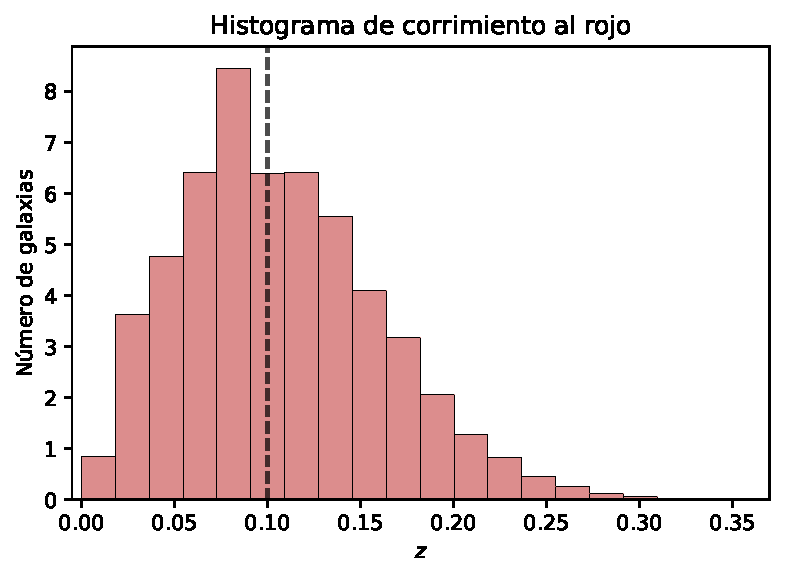
\includegraphics[width=0.9\linewidth]{hist_z.pdf}
\caption{Distribución del redshift de la muestra de galaxias.}
\label{fig:hist_z}
\end{figure}

Al analizar la distribución del redshift de la muestra preliminar (Figura \ref{fig:hist_z}), se observa que la mayor densidad de galaxias se encuentra alrededor de $z \sim 0.1$. Esto es coherente con las características del SDSS, que asegura la completitud del muestreo espectroscópico hasta ese valor de redshift.

\subsection{Aplicación de la Corrección K}

Para calcular las magnitudes absolutas, se utilizaron las Correcciones K en los distintos filtros del SDSS para dos redshifts de referencia: $z = 0.0$ y $z = 0.1$. Estas correcciones se muestran en la Figura \ref{fig:corrk}.

\begin{figure*}[t]
\centering
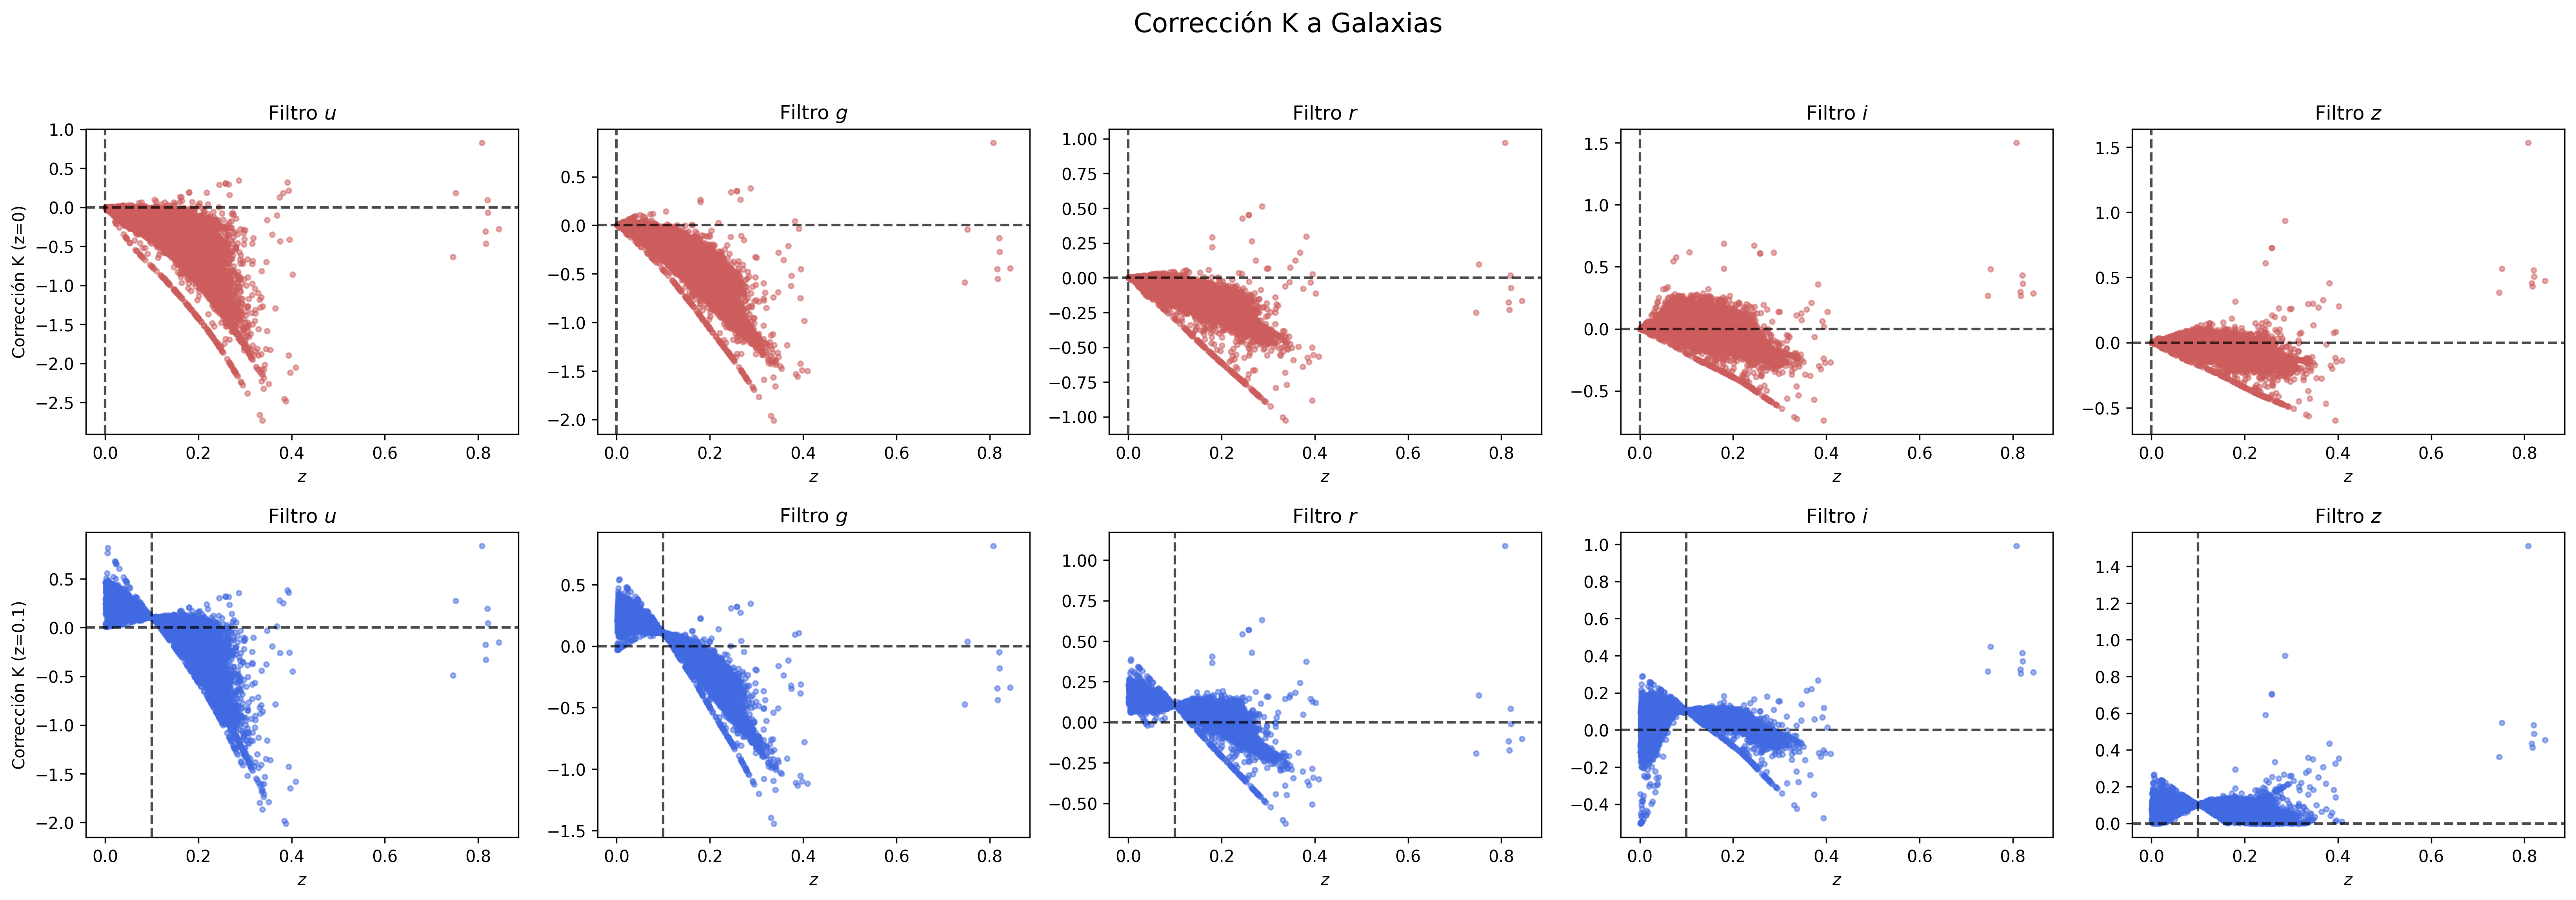
\includegraphics[width=0.9\textwidth]{corrk_combined.png}
\caption{Correcciones K en diferentes filtros para $z = 0.0$ (marco de reposo actual) y $z = 0.1$ (marco de reposo del pico de la muestra).}
\label{fig:corrk}
\end{figure*}

El hecho de que las correcciones a $z=0$ se aproximen a cero cuando $z \to 0$ es un resultado esperado, ya que la galaxia se está comparando con su propia SED en reposo. Sin embargo, al usar una corrección K a $z=0.1$, aquellas galaxias con $z \approx 0.1$ no tienen una corrección nula, sino un valor cercano a cero, lo que implica una corrección para llevar la magnitud al valor actual. Considerando que la muestra tiene un pico en $z \sim 0.1$, se decidió emplear la corrección K con referencia a $z = 0.1$ para mitigar la dispersión de la muestra alrededor de su centro de redshift principal.

La magnitud absoluta se calculó mediante la siguiente expresión, incluyendo la corrección K:
\begin{equation}
M = m - \mu - K_{z} + \text{corr}_{AB} - \text{ext}
\label{eq:Mabs}
\end{equation}
Donde $M$ es la magnitud absoluta, $m$ la magnitud aparente, $\mu$ el módulo de distancia, $K_{z}$ la corrección K aplicada en el filtro, $\text{corr}_{AB}$ la corrección al sistema AB y $\text{ext}$ la extinción.

La Figura \ref{fig:hist_m} muestra la distribución de galaxias según su magnitud absoluta calculada. La caída en el número de galaxias hacia las magnitudes más débiles (menor luminosidad) es una clara evidencia de los efectos de incompletitud de la muestra debido al sesgo de Malmquist.

\begin{figure}[h]
\centering
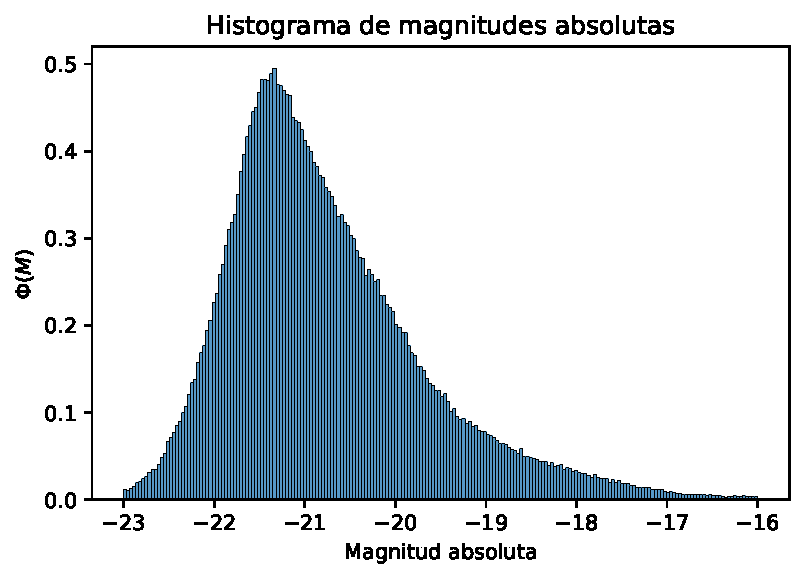
\includegraphics[width=0.9\linewidth]{hist_mag_abs.pdf}
\caption{Histograma de la magnitud absoluta en el filtro $r$ de la muestra de galaxias.}
\label{fig:hist_m}
\end{figure}

\subsection{Determinación de la Función de Luminosidad}

Para contrarrestar el sesgo de Malmquist visible en la Figura \ref{fig:hist_m}, se empleó el Método del Volumen Máximo ($V_{\text{max}}$). Se utilizó una cosmología plana $\Lambda$CDM con parámetros ($H_0 = 70\, \text{km/s/Mpc}$, $\Omega_m = 0.3$, $\Omega_{\Lambda} = 0.7$).

El volumen máximo se define como la integral del elemento de volumen comóvil ($dV_C$) a lo largo de la línea de visión dentro de los límites de redshift del sondeo ($\Omega$):
\begin{equation}
V_{\text{max}} = \Omega \frac{c}{H_0} \int_{z_{min}}^{z_{max}} \frac{D_M^2(z)}{\sqrt{\Omega_m(1+z)^3+\Omega_{\Lambda}}} dz
\label{eq:vol}
\end{equation}
donde $D_M(z)$ es la distancia comóvil.

La Figura \ref{fig:volm} ilustra el crecimiento del $V_{\text{max}}$ con el redshift. Este aumento significativo es el factor clave para corregir el sesgo de Malmquist, ya que asigna un mayor peso a las galaxias intrínsecamente débiles que solo podrían haber sido observadas en un volumen pequeño.

\begin{figure}[h]
\centering
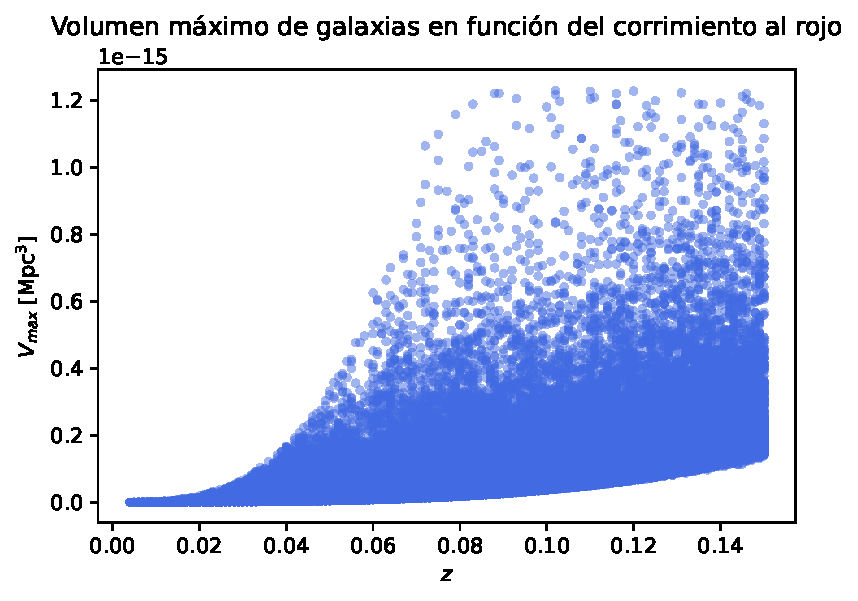
\includegraphics[width=0.9\linewidth]{volm.pdf}
\caption{Volumen comóvil máximo en función del redshift para la cosmología $\Lambda$CDM adoptada.}
\label{fig:volm}
\end{figure}

La función de luminosidad corregida, $\Phi(M)$, fue construida mediante un histograma de 20 bins en el rango de magnitudes absolutas $(-23, -16)$, donde cada bin se ponderó por el factor $1/V_{\text{max}}$. La Figura \ref{fig:phi_m} muestra $\log_{10}(\Phi(M))$ resultante, en la que se observa que la caída en el extremo débil de las magnitudes ha desaparecido, confirmando la mitigación del sesgo de Malmquist.

\subsection{Ajuste de la Función de Schechter}

Para el ajuste de la función de Schechter a $\log_{10}(\Phi(M))$, se empleó la versión logarítmica de la Ecuación \ref{eq:log_schechter}:

\begin{equation}
\log_{10}(\phi) = \log_{10}(A) - 0.4(M-B)C - \frac{1}{\ln(10)}10^{-0.4(M-B)}
\label{eq:log_schech}
\end{equation}
donde las variables de ajuste son $A = \phi^*0.4\ln(10)$, $B = M^*$ y $C = 1 + \alpha$.

El ajuste arrojó los siguientes valores para los parámetros logarítmicos $(A, B, C) = (20.6, -20.8, -0.1987)$. Al convertir estos resultados a los parámetros característicos de Schechter, se obtuvieron: $(\phi^*, M^*, \alpha) = (22.36, -20.85, -1.199)$.

Al comparar estos resultados con los obtenidos por \citet{2001BlantonFUNLUM} para el SDSS, $(\phi^*, M^*, \alpha) = ((1.46 \pm 0.12)\times 10^{-2}, -20.83 \pm 0.03, -1.20 \pm 0.03)$, se observa una excelente concordancia en los valores de la magnitud característica $M^*$ y el índice de pendiente $\alpha$. La gran diferencia en el valor de $\phi^*$ (densidad de normalización) se atribuye a una falta de normalización de las constantes cosmológicas ($H_0/c$) en este trabajo, ya que el enfoque se centró en la forma de la curva.

El ajuste de la función de Schechter superpuesto a la función de luminosidad determinada se presenta en la Figura \ref{fig:phi_schechter}, mostrando una excelente concordancia.

\begin{figure}[h]
\centering
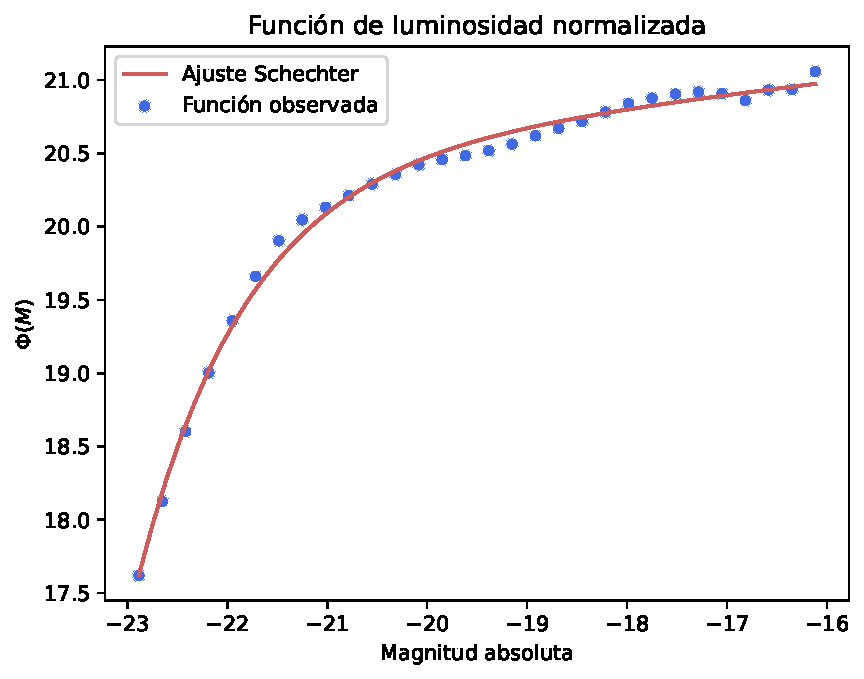
\includegraphics[width=\linewidth]{funcion_lum.pdf}
\caption{Función de luminosidad en el filtro $r$ determinada por el método $V_{\text{max}}$ (histograma) y la función de Schechter ajustada (línea).}
\label{fig:phi_schechter}
\end{figure}

\section{Conclusiones}

El análisis realizado permitió determinar la función de luminosidad de galaxias del SDSS en el filtro $r$ utilizando el Método del Volumen Máximo y mitigar eficazmente el Sesgo de Malmquist. La función de Schechter ajustada a los datos no paramétricos arrojó parámetros clave ($M^*$ y $\alpha$) que son consistentes con los valores reportados en la literatura, validando la metodología empleada.

Se concluye que para trabajar con muestras de redshifts bajos como el SDSS, la selección de la Corrección K referida al redshift central de la muestra ($z \sim 0.1$) es una estrategia apropiada para minimizar los efectos de dispersión y obtener una Función de Luminosidad robusta.






\bibliographystyle{plainnat}
\bibliography{bibliografia}

\end{document}